\section{Basic Principles}
\subsection{Bra and ket notation}

A state vector

\begin{equation}
    \boldsymbol{x} = \begin{bmatrix} x_0 \\ x_1 \\ \vdots \\ x_{n-1} \\ x_n \end{bmatrix} \; ,
\end{equation}

is represented with the Dirac bra-ket notation as

\begin{equation}
    \boldsymbol{x} = \ket{x} = \begin{bmatrix} x_0\\ x_1 \\ x_2 \\ \dots \\ \dots \\ x_{n-1} \end{bmatrix} \; ,
\end{equation}

and the conjugate transpose

\begin{equation}
  \boldsymbol{x}^{\dagger} = \bra{x} = \begin{bmatrix} x_0^* & x_1^* & x_2^* & \dots & \dots & x_{n-1}^* \end{bmatrix} \; .
\end{equation}

With another state vector $\ket{y}$ we have the definition of the inner product

\begin{equation}
    \bra{y}\ket{x} = \sum_{i=0}^{n-1} y_i^*x_i=y_0^*x_0+y_1^*x_1+\dots + y_{n-1}^*x_{n-1} \; .
\end{equation}

and the outer product

\begin{equation}
    \ket{y}\bra{x} = \begin{bmatrix}
        y_{0}^*x_0 & y_{1}^*x_0 & \dots & y_{n-1}^*x_0 & y_{n}^*x_0 & \\y_{0}^*x_{1} & y_{1}^*x_{1} & \dots & y_{n-1}^*x_{1}  &  y_{n}^*x_{1} & \\ \vdots & \vdots & \ddots & \vdots & \vdots \\y_{0}^*x_{n-1} & y_{1}^*x_{n-1} & \dots & y_{n-1}^*x_{n-1} & y_{n}^*x_{n-1} & \\y_{0}^*x_{n} & y_{1}^*x_{n} & \dots & y_{n-1}^*x_{n} & y_{n}^*x_{n}
    \end{bmatrix}
\end{equation}

\subsection{The Qubit}

The most basic piece of information in quantum computing is the qubit, a quantum state with two different states. The standard orthonormal basis states of a qubit is as follows:

$$ \left | 0 \right > = \begin{bmatrix}
    1 \\ 0
\end{bmatrix} \; \space \; \left | 1 \right > = \begin{bmatrix}
    0 \\ 1
\end{bmatrix}$$

This means that the state can only be measured to be in state $\left | 0 \right >$ or $\left | 1 \right >$. Before measurement, however, the state of a qubit can be a superposition of the computational basis states. Which can be described as a linear combination of the two basis states:

$$\left | \psi \right > = \alpha \left | 0 \right > + \beta \left | 1 \right > = \begin{bmatrix}
    \alpha \\ \beta
\end{bmatrix}\; ,$$

where both $\alpha, \beta \in \mathbb{C}$ and with the normalization condition $\lvert\alpha\rvert + \lvert\beta\rvert = 1$. It is usefull to visualize the qubit as a sphere of possible states it can be in, called the Bloch sphere.

\begin{figure}[H]
    \centering
    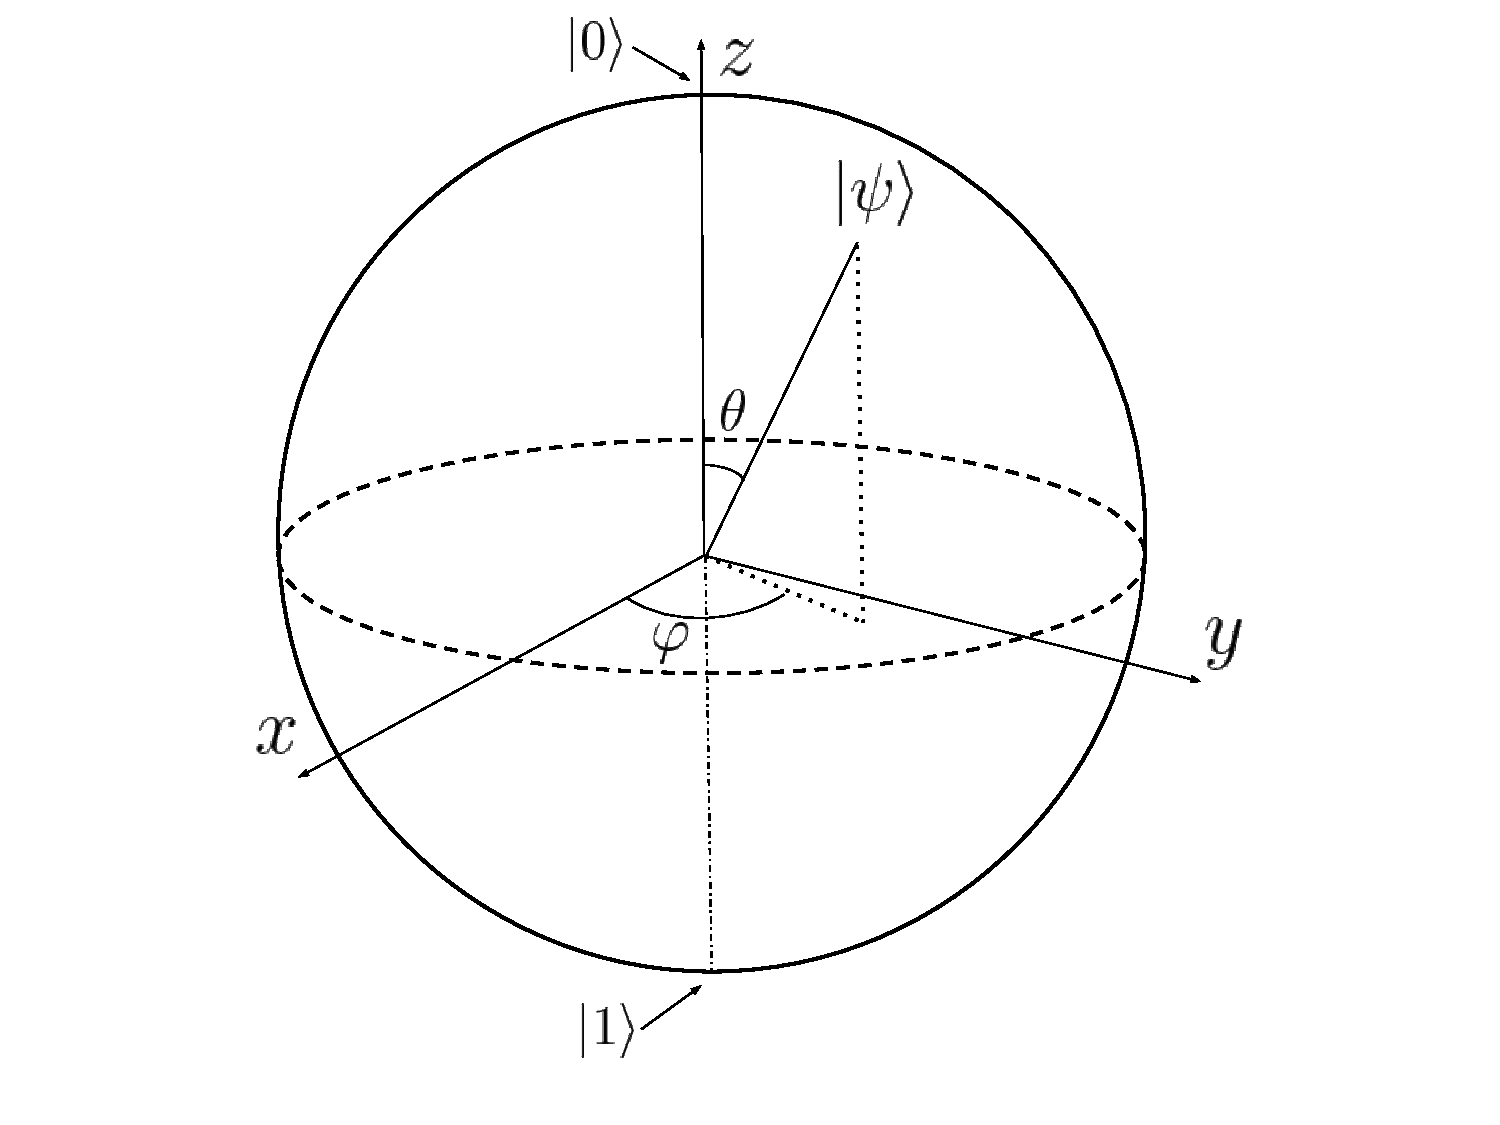
\includegraphics[width=\textwidth]{Figures/Drawn/bloch pshere.pdf}
    \caption{The possible states of a single qubit represented by a sphere with the apexes being the computational basis states.}
    \label{fig:blochsphere}
\end{figure}

Since we have the restriction $\lvert\alpha\rvert + \lvert\beta\rvert = 1$, the two complex values $\alpha$ and $\beta$ only contribute to two degrees of freedom, resulting in the surface of the Bloch sphere, \ref{fig:blochsphere}, as the state space of the single qubit. 
\subsection{Multi-Qubit States}

Bringing in another qubit will give us more possible measured outcomes. Therefor our computational basis needs to be expanded, encompassing every possible combination. This is done by tensor product of the possible single qubit measurements. For a two-qubit system we then have

\begin{gather}
\begin{aligned}\label{eq:twoqubit}
    \ket{0} \otimes \ket{0} = \begin{bmatrix} 1 \\ 0 \end{bmatrix} \otimes \begin{bmatrix} 1 \\ 0 \end{bmatrix} &=  \begin{bmatrix} 1 \\ 0 \\ 0 \\ 0\end{bmatrix} \\
    \ket{1} \otimes \ket{0} = \begin{bmatrix} 0 \\ 1 \end{bmatrix} \otimes \begin{bmatrix} 1 \\ 0 \end{bmatrix} &=  \begin{bmatrix} 0 \\ 1 \\ 0 \\ 0\end{bmatrix} \\
    \ket{0} \otimes \ket{1} = \begin{bmatrix} 1 \\ 0 \end{bmatrix} \otimes \begin{bmatrix} 0 \\ 1 \end{bmatrix} &=  \begin{bmatrix} 0 \\ 0 \\ 1 \\ 0\end{bmatrix} \\
    \ket{1} \otimes \ket{1} = \begin{bmatrix} 0 \\ 1 \end{bmatrix} \otimes \begin{bmatrix} 0 \\ 1 \end{bmatrix} &=  \begin{bmatrix} 0 \\ 0 \\ 0 \\ 1\end{bmatrix} \; ,  
\end{aligned}
\end{gather}
which then is a orthonormal basis for our new two-qubit system. To simplify writing, the tensorproduct between states are often written as

\begin{gather}
\begin{aligned}
    \ket{0} \otimes \ket{0} &= \ket{00} \\
    \ket{1} \otimes \ket{0} &= \ket{10} \\
    \ket{0} \otimes \ket{1} &= \ket{01} \\
    \ket{1} \otimes \ket{1} &= \ket{11} \; .
\end{aligned}
\end{gather}

Adding more qubits is simple. For each additonal qubit one tensormulitply the basis with the single-qubit basis, resulting in a $2^N$ possible measured states of the system. 
\subsection{Unitary Operators}

Unitary operators are used to transform a state to another. They are called unitary because of the condition:

\begin{equation}\label{eq:unitarydef}
    UU^* = U^*U = I \; ,
\end{equation}

where $I$ is the identity matrix of the same size as $U$. This condition is necessary such that the transformations doesn't change the size of the state vector. The unitary matrices applied to a state are often referred to as quantum gates, or just gates, as taken from logical gates in classical computing. For completeness we will give a explanation of all the gates used in this thesis:

The identity matrix does not transform a qubit, but it is an unitary matrix.

\begin{flalign}\label{eq:identity_matrix}
\textbf{Identity}\text{:} &&
 I = \begin{bmatrix}
        1 & 0 \\ 0 & 1
    \end{bmatrix}\; .&&
\end{flalign}

The Pauli spin matrices have applications outside of quantum computing and go by several different names, some which explain better what they do to a quantum bit. The first one is the

\begin{flalign}\label{eq:notgate}
\textbf{NOT Gate}\text{:} &&
 \sigma_x = \begin{bmatrix}
        0 & 1 \\ 1 & 0
    \end{bmatrix}\; ,&&
\end{flalign}

which rotates the state $\pi$ radians around the x-axis, also called bit flip gate because it flips $\left | 0 \right > $ to $\left | 1 \right >$. The

\begin{flalign}\label{eq:paulY}
\textbf{Pauli Y}\text{:} &&
 \sigma_y = \begin{bmatrix}
        0 & -i \\ i & 0
    \end{bmatrix}&&
\end{flalign}

rotates around the y-axis $\pi$ radians. While the

\begin{flalign}\label{eq:phaseflip}
\textbf{Phase Flip}\text{:} &&
 \sigma_y = \begin{bmatrix}
        1 & 0 \\ 0 & -1
    \end{bmatrix}&&
\end{flalign}

rotates around the z-axis $\pi$ radians. For transforming a state into a equal superposition of its opposite on the Bloch sphere we have the:

\begin{flalign}\label{eq:hadamardMatrix}
\textbf{Hadamard}\text{:} &&
    H = \frac{1}{\sqrt{2}}\begin{bmatrix}
        1 & 1 \\ 1 & -1
    \end{bmatrix} \; ,&&
\end{flalign}

which characteristically creates the equal superpositions from the base states:
\begin{alignat}{3}
H \left | 0 \right > = \frac{\left | 0 \right > + \left | 1 \right >}{\sqrt{2}} &
\quad \text{and} \quad &
H \left | 1 \right > = \frac{\left | 0 \right > - \left | 1 \right >}{\sqrt{2}} \; .
\end{alignat}

We also have the
\begin{flalign}\label{eq:phase_gate}
\textbf{Phase Gate}\text{:} &&
 S = \sqrt{\sigma_z} = \begin{bmatrix}
        1 & 0 \\ 0 & i
    \end{bmatrix}\; ,&&
\end{flalign}

which rotates the state $\frac{\pi}{2}$ radians around the z-axis. There are also gates which require a control, an additional qubit which changes the effect of the gate. An example is the

\begin{flalign}\label{eq:controlled_not}
\textbf{Controlled NOT}\text{:} &&
  \textbf{CNOT} = \begin{bmatrix}
        1 & 0 & 0 & 0 \\ 0 & 1 & 0 & 0 \\ 0 & 0 & 0 & 1 \\ 0 & 0 & 1 & 0 
    \end{bmatrix} \; ,&&
\end{flalign} 

which is essentially the identity when the control qubit is in state $\ket{0}$ and a \textbf{NOT} gate when the control qubit is in state $\ket{1}$. Then we have the

\begin{flalign}\label{eq:swap_gate}
\textbf{SWAP Gate}\text{:} &&
  \textbf{SWAP} = \begin{bmatrix}
        1 & 0 & 0 & 0 \\ 0 & 0 & 1 & 0 \\ 0 & 1 & 0 & 0 \\ 0 & 0 & 0 & 1 
    \end{bmatrix}\; ,&&
\end{flalign}

which switches the values of two target qubit.
